\begin{frame}[parent={cmap:software-testing-foundations}, hasprev=false, hasnext=true]
\frametitle{Critério de teste}

\begin{block:fact}{Técnicas e critérios de teste}
\begin{itemize}
	\item Técnicas de teste fornece uma teoria fundamentada de como devemos testar nosso software:
	\begin{itemize}
		\item Quais são as fontes de requisito de teste?

		\item Quais as características das fontes devem ser exploradas?
	\end{itemize}

	\item Entretanto, a fim de testar um software com sucesso, deve ser cuidadosamente especificada como deve ser aplicado as técnicas.
	\begin{itemize}
		\item Queremos dizer com êxito: encontrar erros.
	\end{itemize}
\end{itemize}
\end{block:fact}


\begin{block:fact}{Como aumentar a eficiência}
\begin{itemize}
	\item Os requisitos de teste deve ser estabelecido para explorar não só o que o software deve fazer, mas também o que ele \textbf{não} deve fazer;

	\item Uma medida também deve ser fornecida, de modo que um critério de parada possa ser definido para o teste de atividade.
\end{itemize}
\end{block:fact}
\end{frame}



\begin{frame}[hasprev=true, hasnext=true]
\label{concept:test-criterion}
\frametitle{Critério de teste}

\begin{block:concept}{Definição}
Um critério de teste sistematiza a forma que os requisitos de teste são gerados a partir da fonte de informação(especificação, código fonte, histórico de falhas do banco de dados).
\end{block:concept}

\begin{block:fact}{}
\begin{itemize}
	\item Um critérios de teste fornece uma forma sistemática para selecionar os casos de teste:
	\begin{itemize}
		\item Um critério de teste divide as entradas.
	\end{itemize}

	\item Quando não há falhas encontradas, o critério de teste fornece uma indicação de como os casos de testes devem ser selecionados a fim de estabelecer um alto nível de de confiança de correção do produto.
\end{itemize}
\end{block:fact}


\hfill
\refie{example:test-criterion}{\beamerbutton{Example: Critério de teste example}}
\end{frame}


\begin{frame}
\frametitle{Critério de teste}

\begin{block:fact}{Critério de teste attributes}
\begin{itemize}
	\item Um critério de teste pode ser comparado baseado no custo, eficácia e resistência.
\end{itemize}
\end{block:fact}

\begin{block:fact}{}
    \centering
    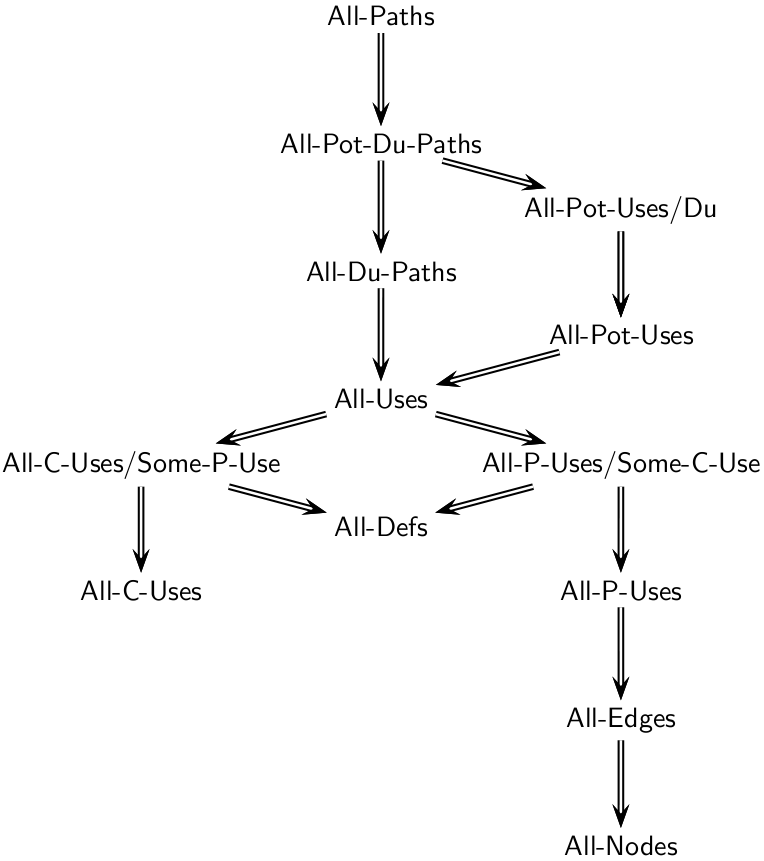
\includegraphics[width=4cm]{teste-de-software/conceitos-basicos/Imagens/subsume-relation}
\end{block:fact}
\end{frame}


\begin{frame}[hasprev=true, hasnext=false]
\frametitle{Critério de teste}

\begin{block:fact}{Teste de cobertura}
\begin{itemize}
	\item Um teste de critério pode ser usado tanto para avaliar o programa em fase de teste ou para avaliação de consistência de um conjunto de teste.
\end{itemize}
\end{block:fact}

\begin{block:concept}{Teste de seleção de critério}
O teste de critério é usado para selecionar casos de teste que avaliem o programa em fase de teste.
\end{block:concept}


\begin{block:concept}{Teste de avaliação de critério}
O teste de critério é utilizado para avaliar os conjuntos de teste.
\end{block:concept}
\end{frame}


% Test cases representing unexpected and invalid input conditions seem to
% have a higher error-detection yield than do test cases for valid input
% conditions~\cite[p. 18]{myers:2004}.
% \begin{itemize}
%	\item Programs must be examined for unwanted side effects~\cite[p. 18]{myers:2004}.
% \end{itemize}

